% !TeX program = lualatex
%%

\documentclass[
	paper=a0,
%	boxstyle= framed, % Boxen mit abgerundeten Ecken, farbigem Titelblock
%	boxstyle=colored % Boxen mit farbigen Hintergrund
%	boxstyle=default % Voreinstellung, keine sichtbare Box, farbiger Titel
%	logofile=example-image, %Falls die Logo Dateien nicht vorliegen
	style=ruled, % Stil für Header/Footer einzeln wählbar über title-style/footer-style, default ist plain
%	logo=head,% Logo im Titelblock anstatt der Fusszeile
%	invert-colors % Orange/Blau im title,footer,logo getauscht. einzeln anwählbar über invert-title-colors,invert-footer-colors,invert-logo-colors
	]{bfhsciposter}
%\usepackage[nswissgerman]{babel}
\usepackage[autostyle]{csquotes}
\newcommand{\tbs}{\textbackslash}
\newcommand{\repl}[1]{<\textit{#1}>}
\let\code\texttt
\newcommand*{\macro}[1]{\code{\tbs#1}}
\let\file\texttt
\let\pck\textsf
\let\cls\textsf
\newcommand{\MVAt}{{\usefont{U}{mvs}{m}{n}\symbol{`@}}}
\usepackage[colorlinks=false]{hyperref}
\usepackage{filecontents}

\begin{filecontents}{\jobname.bib}
@online{bioarchlinux_2022,
	Title = {{B}io{A}rchLinux: bioinformatics community with {A}rch {L}inux \url{https://doi.org/10.7490/f1000research.1119039.1}},
	Author = {Zhang G. and Hu Y.},
	Month = {July},
	url = {https://doi.org/10.7490/f1000research.1119039.1},
	Year = {2022}
}
@online{gitpod_2022,
	Title = {Gitpod an open-source {K}ubernetes application for ready-to-code developer environment \url{https://github.com/gitpod-io/gitpod}},
	Author = {Christian Weichel and Manuel de Brito Fontes},
	Month = {July},
	url = {https://github.com/gitpod-io/gitpod},
	Year = {2018}
}
@online{arch4edu2022,
	Title = {{A}rch {L}inux {R}epository for {E}ducation \url{https://github.com/arch4edu/arch4edu}},
	Author = {Jingbei Li and Carlos Aznarán},
	Month = {September},
	url = {https://github.com/arch4edu/arch4edu},
	Year = {2022}
}
@article{preCICEv2,
  author = {Chourdakis, G and Davis, K and Rodenberg, B and Schulte, M and Simonis, F and Uekermann,
B},
  title = {{preCICE} v2: A sustainable and user-friendly coupling library},
  journal = {Open Research Europe},
  volume = {2},
  year = {2022},
  number = {51},
}
@article{Kochetal2020Dumux,
title = {Du{M}u\textsuperscript{x} 3 - an open-source simulator for solving
          flow and transport problems in porous media with a focus on model
          coupling},
journal = {Computers \& Mathematics with Applications},
year = {2020},
issn = {0898-1221},
}
\end{filecontents}
\bibliographystyle{plain}

\begin{document}
% \pck{tcolorbox}-Template\\
\title{Virtualization of scientific software based on Arch Linux in GitPod}
\author{
	Carlos A. Aznarán Laos\inst{*}\thanks{caznaranl\MVAt uni.pe}\and
	John J. Leal Gomez\inst{**}\thanks{jlealgom\MVAt unal.edu.co}\and
	Guillermo A. Martínez Girón\inst{**}\thanks{gumartinezg\MVAt unal.edu.co}
}
\institute{
	\inst{*}Universidad Nacional de Ingeniería, Rímac, Lima, Peru
	\inst{**}Universidad Nacional de Colombia, Palmira, Valle del Cauca, Colombia
}
%\inst kann in den Autor und Institutsfeldern genutzt werden um eine Zuordnung zu ermöglichen. Bei Nummerierung ist der Nutzer dafür verantwortlich Konflikte mit \thanks zu vermeiden.
%\titlegraphic{\includegraphics[width=10cm]{example-image}}
\footerqrcode{https://cpp-review-dune.github.io}
\footer{\textbf{Website}: \url{https://github.com/cpp-review-dune}\\
\MVAt arch4edu on Twitter.\\[\baselineskip]}%Fusszeile: Falls neben den Logos andere Angaben erforderlich sind

%Instituts/Sponsorenlogos von links nach rechts
\footergraphics{
	
\includegraphics[height=\height]{cppreviewdune}\quad
	
\includegraphics[height=\height]{arch4edu}\qquad
	
\includegraphics[height=\height]{cactus}\quad
	
\includegraphics[height=\height]{gitpod}\quad
	
\includegraphics[height=\height]{pec3logo}\quad
}

\begin{tcbposter}[
		poster={
				columns=4,
				rows=7,
				spacing=1cm,
				%		showframe, %Gitter einblenden. Für Platzierung häufig hilfreich
			},]

	\begin{posterboxenv}[,BFH-abstract,title=Abstract]{name=intro,column=1,span=4}
		We developed an open source repository hosted on GitHub to use
		scientific software based on the \href{https://archlinux.org}{Arch Linux distribution},
		with an up-to-date software ecosystem that includes
		\href{https://dune-project.org/doc/gettingstarted}{DUNE python bindings},
		\href{https://dumux.org}{DuMu\textsuperscript{x}},
		\href{https://fenicsproject.org}{FEniCS},
		\href{https://www.dealii.org}{deal.II},
		\href{https://gmsh.info}{Gmsh},
		\href{https://precice.org/adapters-overview.html}{preCICE adapters},
		among others.
		Unlike other projects such as
		\href{https://github.com/BioArchLinux}{BioArchLinux}~\cite{bioarchlinux_2022}
		or \href{https://github.com/arch4edu}{Arch Linux for education}~\cite{arch4edu2022},
		we include some tutorials on GitHub Classroom to allow the practice
		to any newcomer.
		Automated deployed and available for free use allowing virtualization inside
		GitPod~\cite{gitpod_2022}.
	\end{posterboxenv}

	\begin{posterboxenv}[BFH-framed, title=C++ Review DUNE]{name=title, row=2, span=2, rowspan=2}
		Teachers and students from Peru, Colombia and Mexico participated in the Dune PDELab course 2021 with the aim of modeling physical phenomena using scientific programming in C++. Arch Linux distribution was choosed since have a lot of up-to-date scientific software, e.g. the Dune modules were packaged in this distribution. Moreover,  available in Arch Linux for Education repository.
		
		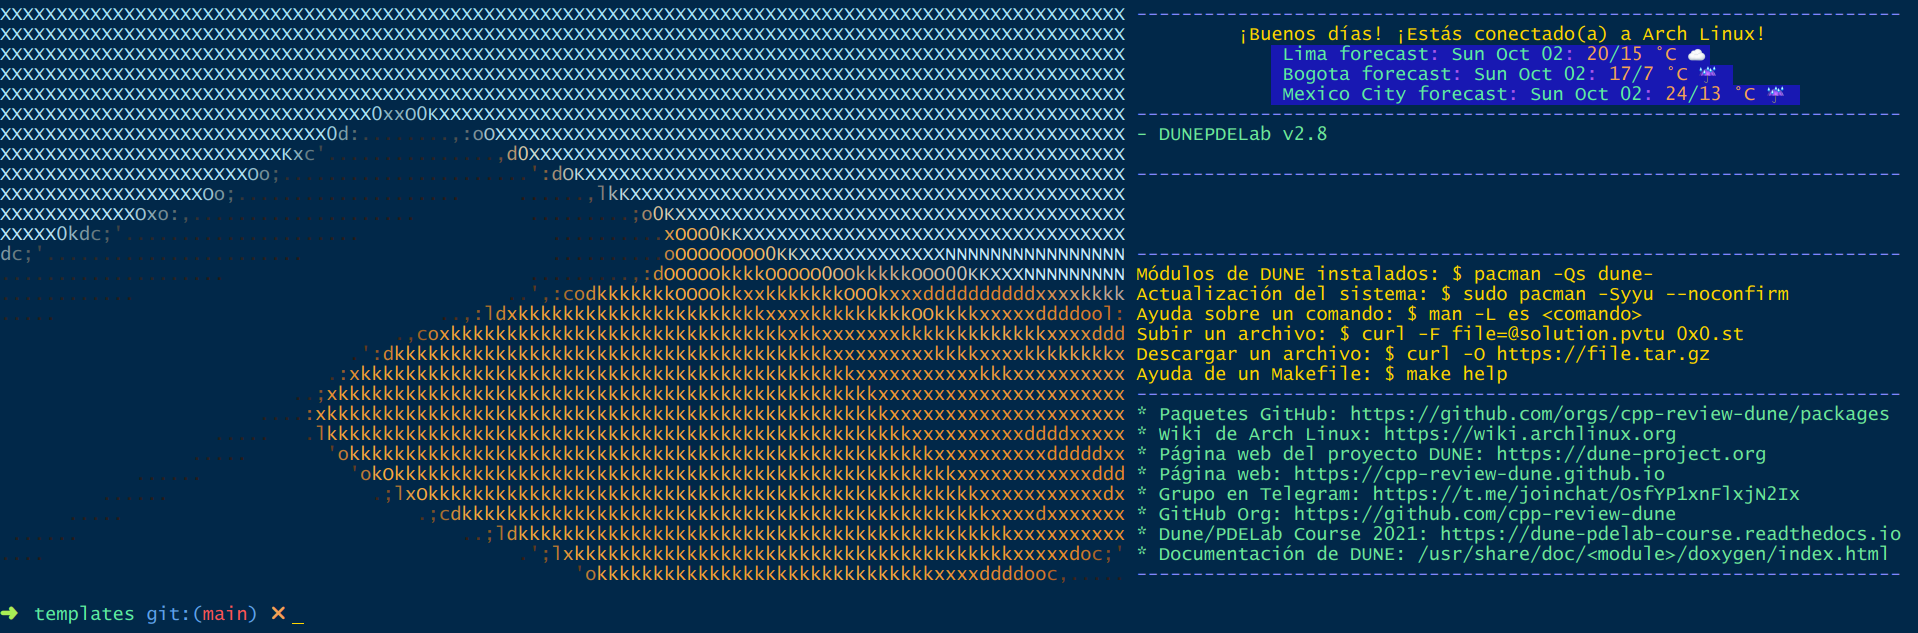
\includegraphics[width=\linewidth]{splash}
		%\captionof{figure}{
		%	C++ Review DUNE says welcome and show useful links to get starting the code inside Gitpod.
		%}
	\end{posterboxenv}

	\begin{posterboxenv}[BFH-framed,title=Tutorials available on Gitpod
		\\
		\url{https://cpp-review-dune.github.io/tutorial}]{name=footer,below=title, span=2, rowspan=4}
		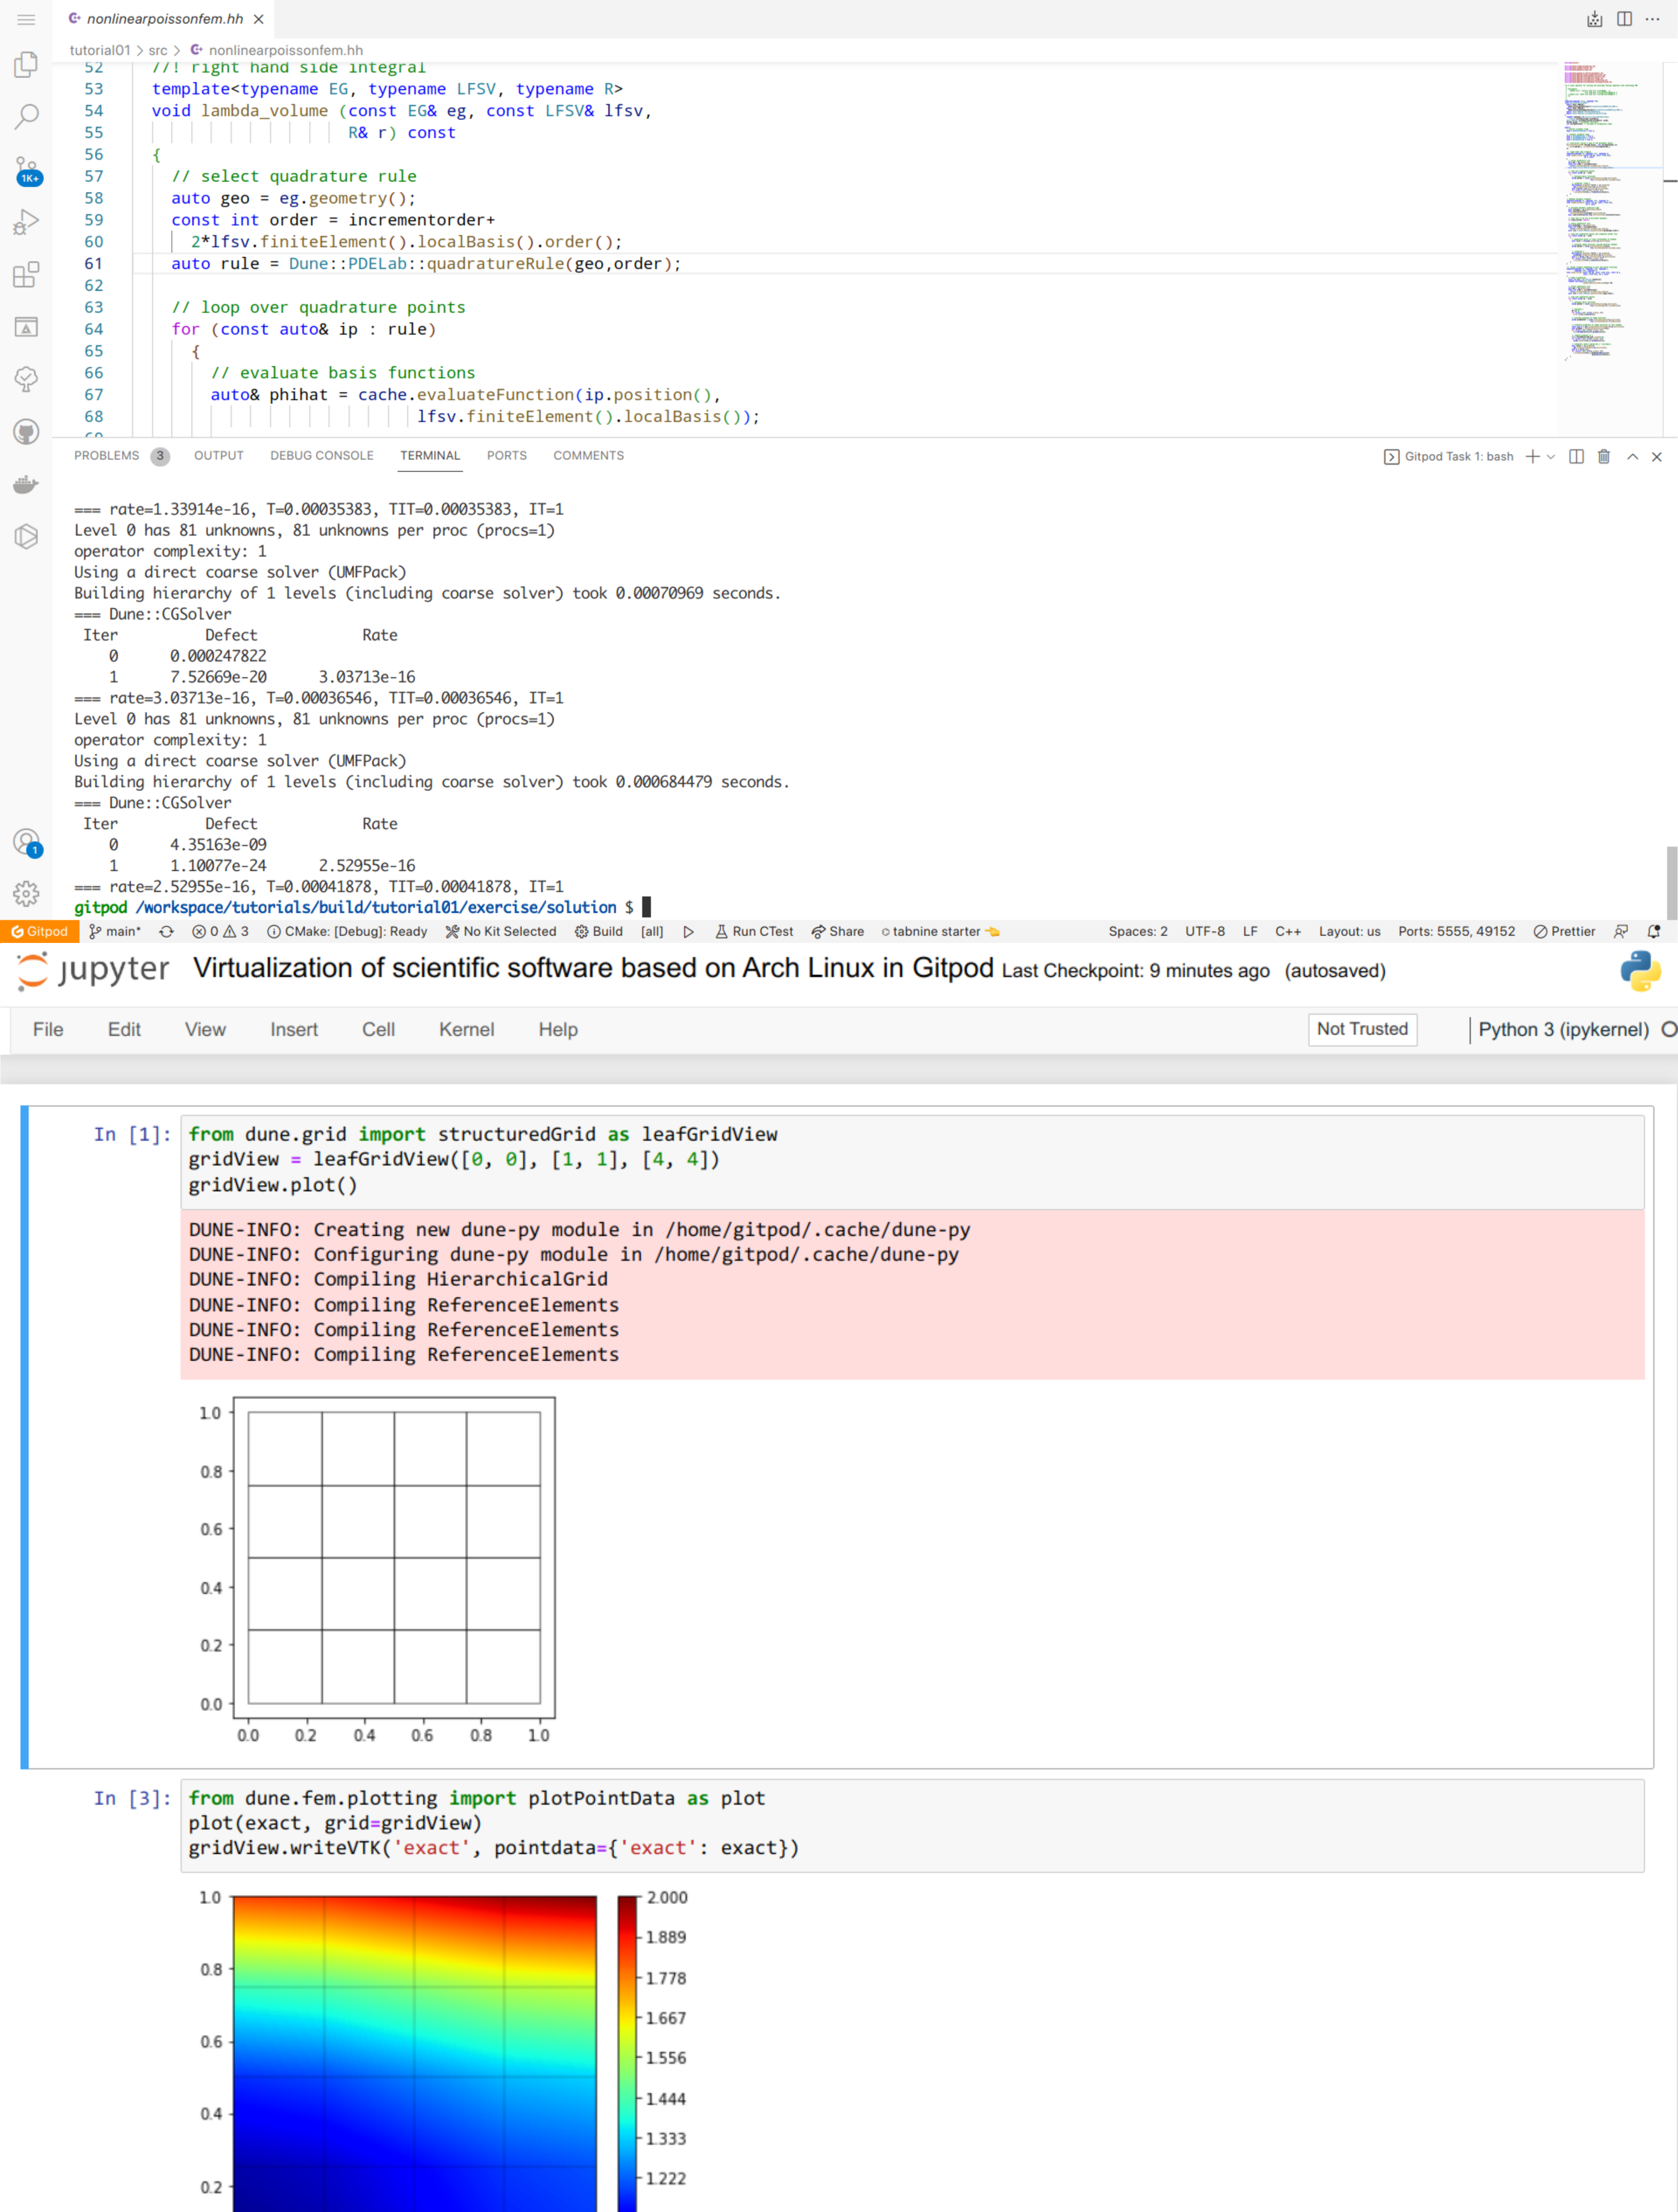
\includegraphics[width=\linewidth]{gitpod_dune}
	\end{posterboxenv}

	\begin{posterboxenv}[title=C++ Review DUNE meets Arch Linux Repository for Education, BFH-framed]{name=colored, column=3, row=2, span=2}
		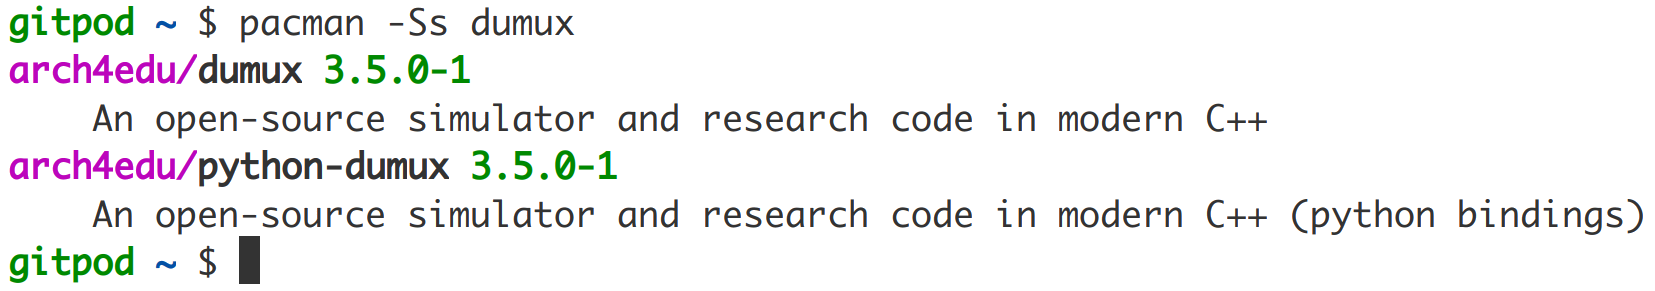
\includegraphics[width=\linewidth]{arch4edu_gitpod}
	\end{posterboxenv}

	\begin{posterboxenv}[BFH-framed]{name=colored-notitle,column=3,row=3, rowspan=2}
		\includegraphics[width=\linewidth]{dumux_2p}
		Example of water contamination due loses leaky oil while parking.
		\[
			v=
			-\frac{1}{\mu}
			K
			\left(\nabla p+\rho g \nabla z\right).
		\]
		$p$ pressure, $K$ absolute permeability,
		$\mu$ viscosity, $\rho$ density.
	\end{posterboxenv}

	\begin{posterboxenv}[BFH-framed]{column=4, below=colored}
		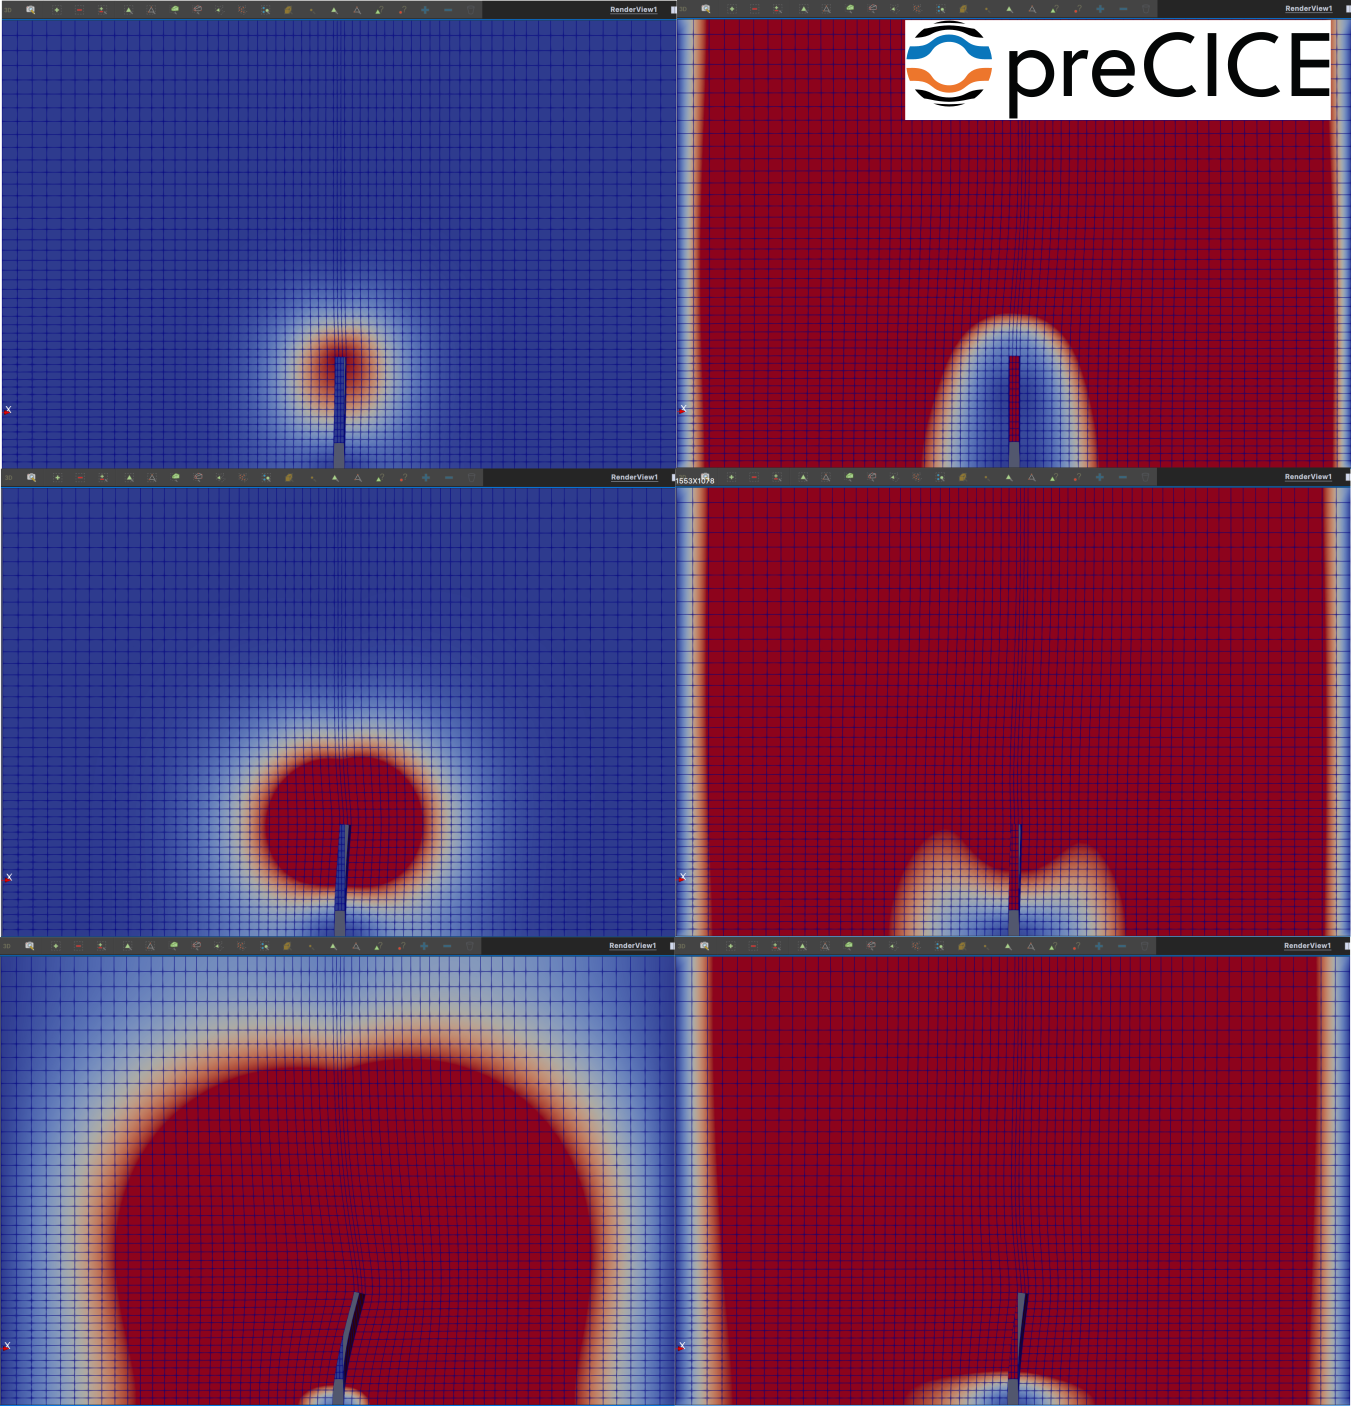
\includegraphics[width=\linewidth]{sequence}
		Example of a fluid-structure interaction, e.g. fluid flowing through a channel in 2D.
	\end{posterboxenv}

	\begin{posterboxenv}[BFH-framed,title=GitHub's Docker registry
		\\
		\url{https://github.com/orgs/cpp-review-dune/packages}]{column=3,span=2,below=row4}
		We use GitHub continuous integration and Docker registry for use enviroment gitpod with  tutorials about Dune Python bindings, DuMux,  Gmsh, preCICE, TeX Live to name a few, also users can run a USB stick or virtualization software
		from \url{sourceforge.net/projects/dune-archiso}
		Another hand, the Dune modules are tested in \url{gitlab.com/dune-archiso/testing/aur/dune-makepkg}. 
	\end{posterboxenv}

	\begin{posterboxenv}[BFH-framed]{name=notitle,column=3,span=2,below=row5}
		\nocite{*}
		\bibliography{\jobname}
	\end{posterboxenv}

\end{tcbposter}

\end{document}